\documentclass[12pt,a4,english,finnish,pdflatex%,handout
]{beamer}
\definecolor{MyGreen}{RGB}{50, 120, 50}
\usecolortheme[named=MyGreen]{structure}

\usepackage{babel}
\usepackage[utf8]{inputenc}
\usepackage[T1]{fontenc}
\usepackage{amsmath,amssymb} 
\usepackage{animate}
\usepackage{multimedia}

\usepackage{natbib}
\bibpunct[: ]{(}{)}{,}{}{}{;}

\usepackage{tikz}

\usepackage{tipa}

\usepackage{hyperref}

\setbeamertemplate{navigation symbols}{}

\graphicspath{{figures/}}

\setlength{\leftmargini}{0pt}
\setlength{\leftmarginii}{1em}

\newcommand{\kommentti}[1]{
  {\bf[#1]}
}



\begin{document}
\title{
Ideas for ((Un)Real) Speech} 
\author{Pertti Palo} 
\date{16 June 2024}

\frame{\titlepage
} 

\frame{%\frametitle{Land acknowledgement}
\includegraphics[width=\textwidth]{land_acknowledgement_statement.pdf}
}

% \frame{\frametitle{Land acknowledgement}
% We wish to acknowledge and honor the Miami, Delaware, Potawatomi, Kickapoo, and
% Shawnee people, on whose ancestral homelands I have worked on this presentation.
% }

\frame{\frametitle{Notes on content}
  \begin{itemize}
  \item I want to keep this a safe space of mutual respect.
  \item There may be discussion of topics such as colonization, oppression,
  pejoratives, etc. in this workshop, but if you want them or any other topics
  kept out, we will do our best to do so.
  \item Touching on 'political' topics will be inevitable though.
  \end{itemize}  
}

% \frame{\frametitle{Outline}
%     \begin{itemize}
%     \item {Ideas for Fantastic ((un)real) Speech}
%   \begin{itemize}
%     \item Who's this guy?
%     \item What we'll do
%     \item  {Dragon speech!}
%     \item  {Bird people!}
%     \item  {Speech and magic!}
%     \item  {You get to have your own take on this - It's a workshop}
%   \end{itemize}
%   \end{itemize}
% }

\frame{\frametitle{Who's this guy?}
  \begin{columns}
    \begin{column}{5cm}
      \includegraphics[width=\columnwidth]{uti_eva.png}
    \end{column}
    \begin{column}{5cm}
      \begin{itemize}
      \item Pertti Palo
      \item I've got a couple of degrees (loosely speaking) in engineering.
      \item I've also got a PhD in Phonetics.
      \item I have no formal qualifications in Borrowing a Language, but I do
      know a lot about speech production, and\ldots
      \end{itemize}
    \end{column}
  \end{columns}
} 

\frame{\frametitle{I do have some background}
\begin{itemize}
  \item I am not a text linguist but rather a phonetician and a speech
  researcher.
  \item When I say 'language' I mainly mean spoken language today. 
  \item Besides a speech researcher with 20+ years of experience, I've been an
  RPG enthusiast for 30+ years. 
  \item Recently I've also started training as an oral storyteller which has
  some interesting connections with RPGs and science.
\end{itemize}
}

\frame{\frametitle{What we'll do}
\begin{itemize}
  \item I'll talk about dragon speech if you want me to.
  \item If there's not too many of us, we'll go round the table and talk about
  the projects each of you is working on, concentrating on questions about
  speech and how it interacts with world and story.
  \item I've got some ideas to play around with on the next slides, but we
  don't need to look at those. 
\end{itemize}
}

\frame{\frametitle{Dragon speech}
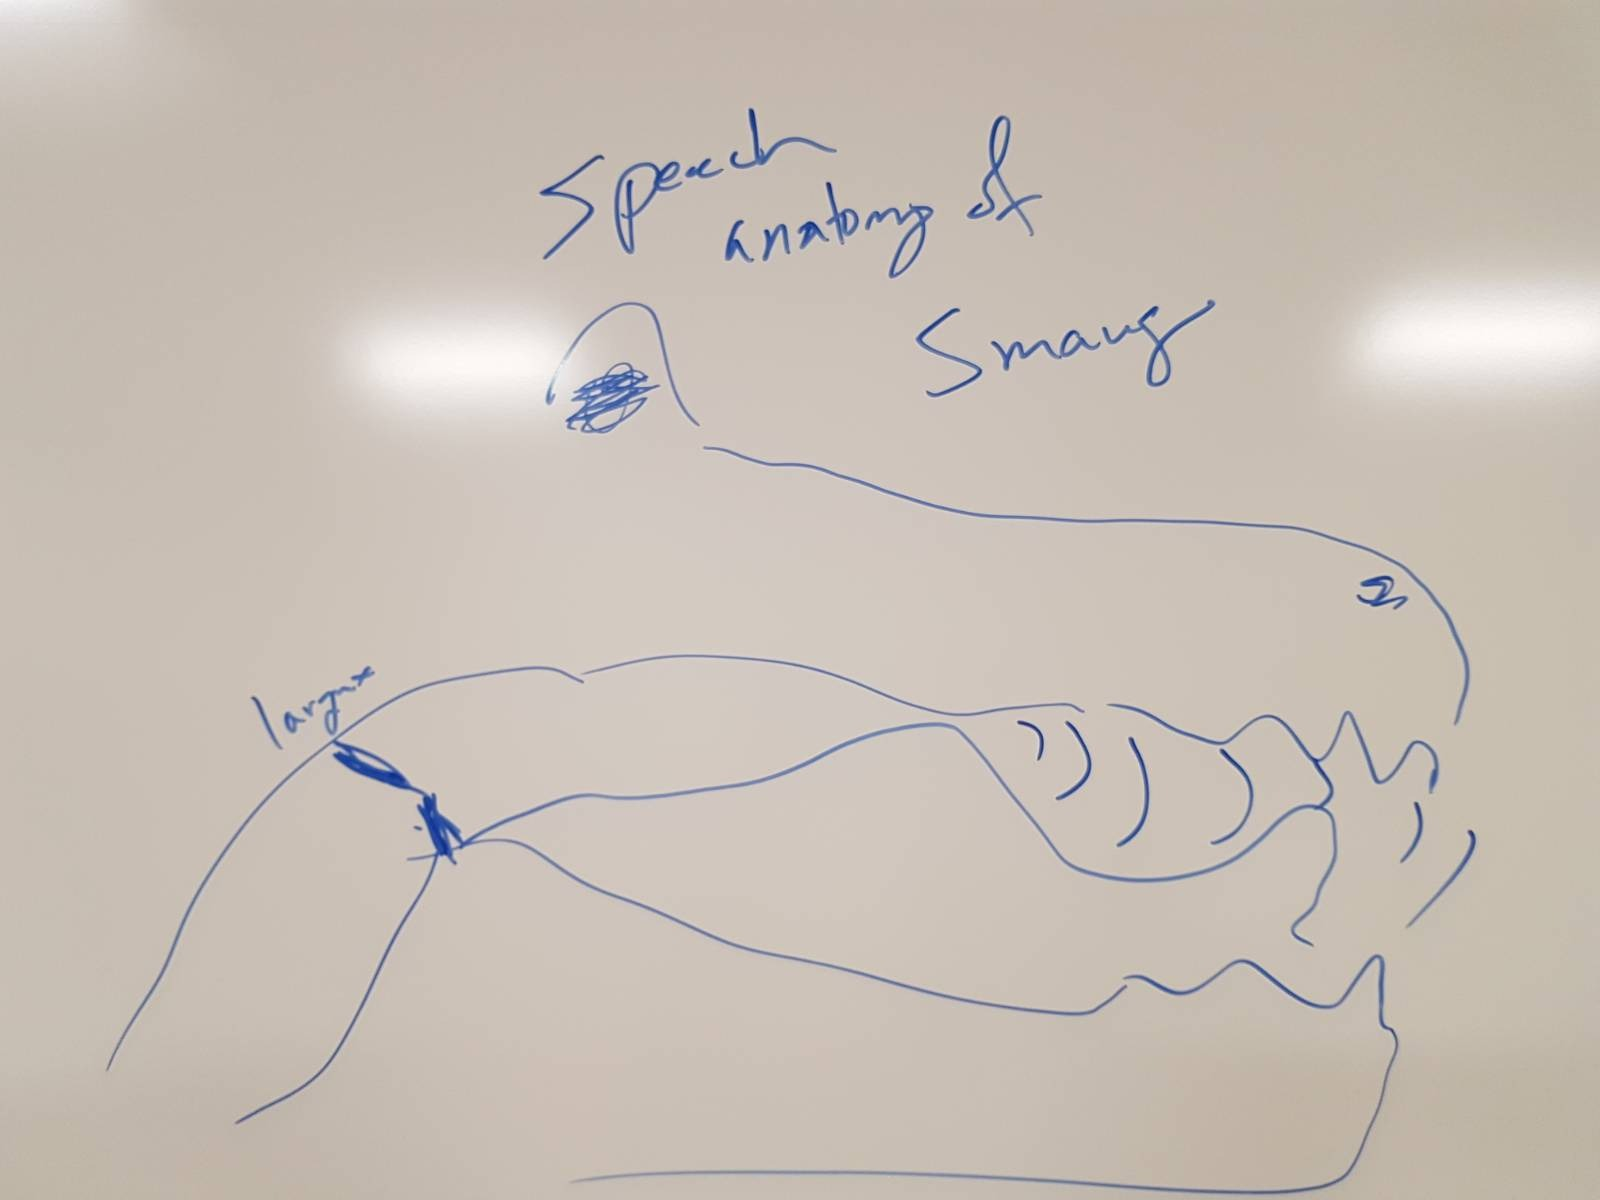
\includegraphics[width=.95\textwidth]{smaug.jpeg}
Image courtesy of Prof Steven Lulich.
}

\frame{\frametitle{Ideas to play around with}
\begin{itemize}
  \item Dragon speech and physics (such as they are) and the consequences to the
  world or story.
  \item Humanoids who do not use sound as a means of communication (and possibly
  can not perceive it).
  \item The base code of reality being a spoken (/speakable) programming
  language.
  \item Social and/or physical environment of speech and language in a world or
  story.
\end{itemize}
}


\frame{\frametitle{Some more ideas to play around with}
\begin{itemize}
  \item If the world is magical, language can be too: 
  \begin{itemize}
    	\item Unholy, vowel rich language (cf. Moorcock): hääyöaie (i.e. you can
    	do this with Finnish)
    	\item "Guttural, evil language" was not a great idea to start with.
  \end{itemize}  
  \item Homophone words (think 'for' and 'four') and homonyms (see
  \url{https://en.wikipedia.org/wiki/Homonym} for details) and other plays on words
  can be part of a story ("Pedo mellon a minno.")
  \begin{itemize}
    \item Mix this with dialects and you can produce a pretty solidly confusing
    situation.
    \item Working these into game play may not be the easiest though.  
  \end{itemize}
  \item Whistled and drummed languages (they are a real thing in the real world)
  \item Singing
\end{itemize}
}

\frame{\frametitle{Acknowledgements}

\begin{itemize}
  \item Again, the people who's ancestral land I have worked on.
  \item Wikipedia is a lovely thing.
  \item All the good folk mentioned in passing and some that I've forgotten.
  \item Copyrighted work remains the property of the legal copyright holders.
  \item Excellent participants of the previous versions of this workshop
  (Indiana ComicCon 2022, Ropecons 2022 \& 2023).
  \item My work has been supported by a grant from Säätiöiden Post Doc pooli
  (they don't have an English name) / The Emil Aaltonen foundation.
  \end{itemize}
}


\end{document}

